\section{Phénoménologie des différents modes de transfert thermique}

    \subsection{Les trois modes de transfert thermique}

        \subsubsection{Conduction thermique}

            C'est un transfert thermique des zones les plus chaudes vers les plus froides \textbf{sans mouvement macroscopique du milieu}. C'est le seul transfert thermique possible dans \textbf{un solide opaque}. La Figure~\ref{fig:exemple_transfert_thermique_conduction} donne un exemple.

            \begin{figure}
                \centering
                \tikzsetnextfilename{exemple_transfert_thermique_conduction}
                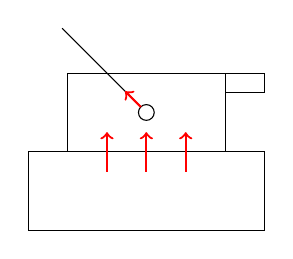
\begin{tikzpicture}[scale=1]  
    
                    \draw (0,0) rectangle++(3,1);
                    \draw (0.5,1) rectangle++(2,1);
                    \draw (2.5,1.75) rectangle++(0.5,0.25);
                    \draw [->, red, thick] (1.5,0.75) --++ (0,0.5);
                    \draw [->, red, thick] (1,0.75) --++ (0,0.5);
                    \draw [->, red, thick] (2,0.75) --++ (0,0.5);
                    \draw [color=black,smooth] (1.5,1.5) circle (0.1);
                    \draw (1.43,1.57) --++ (-1,1);
                    \draw [->, red, thick] (1.43,1.57) --++ (-0.2,0.2);
    
                \end{tikzpicture}
                \caption[Exemple d'un transfert thermique par conduction.]{Exemple d'un transfert thermique par conduction : casserole sur une plaque à induction avec une cuillère.}
                \label{fig:exemple_transfert_thermique_conduction}
            \end{figure}

        \subsubsection{Convection thermique}

            C'est un transfert thermique dû aux mouvement macroscopique du milieu. C'est le transfert dominant \textbf{dans les fluides}, il peut être forcé ou naturel. La Figure~\ref{fig:exemple_transfert_thermique_convection} donne un exemple.

            \begin{figure}
                \centering
                \tikzsetnextfilename{exemple_transfert_thermique_convection}
                \begin{tikzpicture}[scale=1]  
    
                    \draw [fill=blue] (0,0) rectangle++(3,1);
                    \draw (0,1) --++ (0,0.25);
                    \draw (3,1) --++ (0,0.25);
                    \draw [color=yellow,smooth,decoration={markings, mark=at position 0.625 with {\arrow{<}}},
                    postaction={decorate}] (0.75, 0.5) circle (0.25);
                    \draw [color=yellow,smooth,decoration={markings, mark=at position 0.625 with {\arrow{<}}},
                    postaction={decorate}] (2.25, 0.5) circle (0.25);
                \end{tikzpicture}
                \caption[Exemple d'un transfert thermique par convection.]{Exemple d'un transfert thermique par convection : mouvements naturels dans un bassin d'eau chaude.}
                \label{fig:exemple_transfert_thermique_convection}
            \end{figure}

        \subsubsection{Rayonnement thermique}

            Tout corps opaque chauffé à une température $T$ rayonne une puissance surfacique
            \begin{equation}
                \frac{\d P}{\d S}\propto T^{4}.
            \end{equation}
            Un exemple est le rayonnement électromagnétique. Le rayonnement se propage dans un milieu transparent (notamment dans le vide).

        \begin{example}[Chauffage central]
            La pompe électrique implique une convection forcée dans le circuit. Le radiateur implique une conduction à travers la paroi, un rayonnement thermique et une convection naturelle du sol vers le plafond.
        \end{example}

        \begin{example}[Feu de cheminée]
            L'écran de verre stoppe le rayonnement.
        \end{example}
    
    \subsection{Le flux thermique surfacique}

        On considère une section infinitésimale $\d S$ avec une normale extérieure $\vec{n}$ et une quantité de chaleur $\delta Q$ qui passe à travers cette surface, voir la Figure~\ref{fig:flux_thermique_surfacique_section}.

        \begin{figure}
            \centering
            \tikzsetnextfilename{flux_thermique_surfacique_section}
            \begin{tikzpicture}[scale=1]  
                % \helpgrid{3}{3}
                \draw [thick] (0,0) ellipse (1cm and 1.5cm) node [below, shift=({0,-0.25})] {$\d S$};
                \draw [color=black,smooth, pattern=north west lines] (0,0) circle (0.25);
                \draw [thick, ->] (0,0)--++(2,0) node [above] {$\vec{n}$};
                \draw [-stealth, double, thick, red!50!black, text=red] (-3, 0)--++(1.5,0) node [above,pos=0.5] {$\delta Q$};
            \end{tikzpicture}
            \caption{Définition du flux thermique surfacique.}    
            \label{fig:flux_thermique_surfacique_section}
        \end{figure}

        \begin{definition}[Puissance thermique et flux thermique surfacique]
            On définit \textbf{la puissance thermique} par 
            \begin{equation}
                P_{\text{th}}=\frac{\delta Q}{\d t},    
            \end{equation}
            qui est une quantité algébrique : si le transfert se fait selon $\vec{n}$, alors $P_{\text{th}}$, et sinon $P_{\text{th}}<0$. ON a $P_{\text{th}}$ et on définit donc \textbf{le flux thermique surfacique} $\varphi$ par
            \begin{equation}
                \boxed{
                    P_{\text{th}}=\iint_{S}\varphi~\d S.
                }
            \end{equation} 
            L'unité de $\varphi$ est \si{\watt\per\metre\squared}.
        \end{definition}

    \subsection{Continuité du flux surfacique}

        On considère le système présenté à la Figure~\ref{fig:continuite_flux_surfacique}.

        \begin{figure}
            \centering
            \tikzsetnextfilename{continuite_flux_surfacique}
            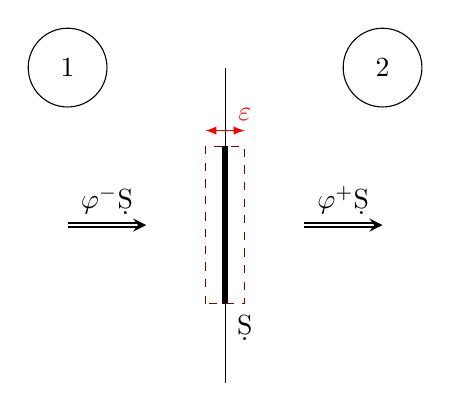
\begin{tikzpicture}[scale=1]  
                % \helpgrid{3}{3}
                \draw (0,-2)--(0,2);
                \draw[thick,line width=2pt] (0,-1)--(0,1) node [below right, pos=0] {$\d S$};
                \draw[dashed, red!50!black] (-0.25,-1) rectangle++ (0.5,2);
                \draw [<->,latex-latex, text=red, color=red] (-0.25,1.2)--++(0.5,0) node [above] {$\varepsilon$};

                \draw [color=black,smooth] (-2,2) circle (0.5) node {1};
                \draw [color=black,smooth] (2,2) circle (0.5) node {2};

                \draw[-stealth, double, thick] (-2,0)--++(1,0) node [above, midway] {$\varphi^{-}\d S$};
                \draw[-stealth, double, thick] (1,0)--++(1,0) node [above, midway] {$\varphi^{+}\d S$};
            \end{tikzpicture}
            \caption{Continuité du flux thermique surfacique.}    
            \label{fig:continuite_flux_surfacique}
        \end{figure}

        Le principe de la thermodynamique sur le tube de volume $\varepsilon\d S$ s'écrit
        \begin{equation}
            \frac{\d U}{\d t}=\varphi^{-}\d S-\varphi^{+}\d S.
        \end{equation}
        Si $\varepsilon\to0$, on a $U\to0$ donc $\frac{\d U}{\d t}\to0$. Ainsi, $\varphi^{-}=\varphi^{+}$ : le flux surfacique est continu.

    \subsection{Hypothèse de l'équilibre thermodynamique local (ETL)}

        S'il existe un transfert thermique, le système est hors d'équilibre. Dans ce cas, \og la\fg~température du système n'est pas définie à l'échelle macroscopique.
        À l'échelle microscopique, on fait donc l'hypothèse de l'ETL. Si $d$ est la distance typique microscopique, $l$ est la distance typique mésoscopique et $L$ la distance typique macroscopique, alors
        \begin{itemize}
            \item $d\ll l$ : on fait un traitement statistique,
            \item $l\ll L$ : la description est locale,
        \end{itemize}
        voir la Figure~\ref{fig:hypothese_etl}.

        \begin{figure}
            \centering
            \tikzsetnextfilename{hypothese_etl}
            \begin{tikzpicture}[scale=1]  
                % \helpgrid{3}{3}
                \draw [thick, smooth] (0,0) ellipse (2cm and 2.5cm);
                \draw [color=black,smooth, pattern=north west lines] (1,-1) circle (0.25) node [above, shift=({0,0.2})] {$\delta V$};
                \draw [stealth-stealth, thick] (2.5, -2.5)--++(0,5) node [right,midway] {$L$};
                \draw [stealth-stealth, thick] (0.75, -1.4)--++(0.5,0) node [below,midway] {$l$};

                \draw [->,-latex] (-5,2) --++ (-0.5,-1);
                \draw [->,-latex] (-5,2) --++ (1.5,0);
                \draw [->,-latex] (-5,2) --++ (0,1.5);
                \draw [->, -stealth, thick] (-5,2) -- (1,-1) node [above, pos=0.4] {$\vec{r}$}; 
            \end{tikzpicture}
            \caption{Hypothèse de l'équilibre thermodynamique local.}    
            \label{fig:hypothese_etl}
        \end{figure}

        On définit $T(\vec{r},t)$ \textbf{la} température du volume mésoscopique $\delta V$ à l'instant $t$. Ainsi, à l'échelle mésoscopique, on a l'hypothèse ETL, et à l'échelle macroscopique, il persiste un déséquilibre.

        